
\section*{CHƯƠNG 2. PHÂN TÍCH HỆ THỐNG}
\setcounter{section}{2}
\setcounter{subsection}{0} %LƯU Ý MỖI LẦN THÊM CHƯƠNG MỚI CẦN THÊM CÂU NÀY ĐỂ RESET THỨ TỰ CỦA SUBSECTON VỀ 1
\setcounter{table}{0} % LƯU Ý SAU MỖI LẦN GỌI BẢNG HAY HÌNH ẢNH PHẢI THÊM CÂU NÀY ĐỂ RESET THỨ TỰ
\setcounter{figure}{0} %% LƯU Ý SAU MỖI LẦN GỌI BẢNG HAY HÌNH ẢNH PHẢI THÊM CÂU NÀY ĐỂ RESET THỨ TỰ
\addcontentsline{toc}{section}{\numberline{}CHƯƠNG 2. PHÂN TÍCH HỆ THỐNG}
Trong chương này, chúng em sẽ tiến hành phân tích hệ thống cho dự án đề tài "Hệ thống theo dõi và quản lý dữ liệu điện tim" dựa trên các mục tiêu
đã nêu ra trong Mục Đề xuất hệ thống ở Phần mở đầu. Trước tiên bài toán đặt ra ở hệ thống là:
\begin{adjustwidth}{1.5em}{}
\begin{itemize}
  \item Một ứng dụng để có thể giúp người dùng/bệnh nhân theo dõi được những thông tin cần về sức khoẻ tim mạch
  \item Trực quan và tiêu chuẩn hoá những thông tin đo được
    bằng hình ảnh hoặc số liệu để bác sĩ có thể dựa vào đó để đưa ra những đánh giá cho người dùng. Ngoài ra những thông tin này
    có thể hữu ích trong việc theo dõi sức khỏe tim mạch, theo dõi hiệu quả của liệu pháp 
    và hỗ trợ quyết định của người dùng
  \item Quản trị viên sẽ là người có thể phân công bác sĩ để chăm sóc, theo dõi sức khoẻ từ
  xa cho bệnh nhân
\end{itemize}
\end{adjustwidth}
Chi tiết về việc phân tích các yêu cầu hệ thống sẽ được chúng em trình bày ở các chương dưới.
% \newpage
\subsection{Thẻ CRC (Class - Responsibility - Collaboration Card)}

\subsubsection{Thẻ CRC lớp Người dùng}
  \begin{table}[H]
    \caption{\bfseries \fontsize{12pt}{0pt}\selectfont Thẻ CRC lớp Người dùng}
    \centering
    \begin{tabularx}{0.9\textwidth}{X}
      Mặt trước thẻ
    \end{tabularx}
    \begin{tabularx}{0.9\textwidth}{|X|X|}
      \hline
      \textbf{Tên lớp:} Người dùng & \textbf{ID:} 1 \\
      \hline
      \textbf{Mô tả:} Đối tượng mô tả thông tin người dùng & \textbf{Use case liên quan:}  Đăng ký tài khoản, Quản lý tài khoản cá nhân, Xem danh sách bệnh nhân\\
      \hline
      \textbf{Trách nhiệm (Responsibility):} & \textbf{Các lớp liên quan (Collaboration):} \\
      Mô tả thông tin người dùng

      Thêm, sửa, xóa thông tin người dùng 

      Lấy danh sách người dùng

      Lấy thông tin người dùng qua id, tài khoản, chức vụ
      & 
      Tài khoản, Phân công bác sĩ - bệnh nhân
      \\
      \hline
    \end{tabularx}
    \begin{tabularx}{0.9\textwidth}{X}
      Mặt sau thẻ
    \end{tabularx}
    \begin{tabularx}{0.9\textwidth}{|X|X|}
      \hline
      \textbf{Thuộc tính (Attributes):} & \\
      id(uuid) 
      
      account\_id(String)

      username(String)

      birth(Timestamps)

      phone\_number(String)
      & 
      image(String) 
      
      role(Integer) 
      
      created\_at(Timestamps)

      updated\_at(Timestamps)
      \\
      \hline
    \end{tabularx}
    \begin{tabularx}{0.9\textwidth}{|X|}
      \textbf{Relationships} \\
      Generalize:  

      Toàn thể - Bộ phận (Aggregation):
      
      Liên kết (Association): Tài khoản, Phân công bác sĩ - bệnh nhân 
      \\
      \hline
    \end{tabularx}
  \end{table}

  \subsubsection{Thẻ CRC lớp Tài khoản}
  \begin{table}[H]
    \caption{\bfseries \fontsize{12pt}{0pt}\selectfont Thẻ CRC lớp Tài khoản}
    \centering
    \begin{tabularx}{0.9\textwidth}{X}
      Mặt trước thẻ
    \end{tabularx}
    \begin{tabularx}{0.9\textwidth}{|X|X|}
      \hline
      \textbf{Tên lớp:} Tài khoản & \textbf{ID:} 2 \\
      \hline
      \textbf{Mô tả:} Đối tượng mô tả thông tin tài khoản & \textbf{Use case liên quan:} Đăng ký, Đăng nhập/Đăng xuất, Quên mật khẩu, Quản lý tài khoản người dùng \\
      \hline
      \textbf{Trách nhiệm (Responsibility):} & \textbf{Các lớp liên quan (Collaboration):} \\
      Mô tả thông tin tài khoản
      
      Đăng nhập/Đăng xuất hệ thống

      Đăng ký tài khoản

      Quên mật khẩu

      Chỉnh sửa thông tin tài khoản

      Lấy thông tin tài khoản qua email
      & 
      Người dùng, Token đăng nhập
      \\
      \hline
    \end{tabularx}
    \begin{tabularx}{0.9\textwidth}{X}
      Mặt sau thẻ
    \end{tabularx}
    \begin{tabularx}{0.9\textwidth}{|X|}
      \hline
      \textbf{Thuộc tính (Attributes):} \\
      id(String) 
      
      email(String)

      password(String)
      \\
      \hline
    \end{tabularx}
    \begin{tabularx}{0.9\textwidth}{|X|}
      \textbf{Mối quan hệ (Relationships):} \\
      Tổng quát hóa (Generalize):  

      Toàn thể - Bộ phận (Aggregation):   
      
      Liên kết (Association): Người dùng, Token đăng nhập 
      \\
      \hline
    \end{tabularx}
  \end{table}

\subsubsection{Thẻ CRC lớp Tài khoản phê duyệt}
  \begin{table}[H]
    \caption{\bfseries \fontsize{12pt}{0pt}\selectfont Thẻ CRC lớp Tài khoản phê duyệt}
    \centering
    \begin{tabularx}{0.9\textwidth}{X}
      Mặt trước thẻ
    \end{tabularx}
    \begin{tabularx}{0.9\textwidth}{|X|X|}
      \hline
      \textbf{Tên lớp:} Tài khoản phê duyệt & \textbf{ID:} 3 \\
      \hline
      \textbf{Mô tả:} Đối tượng mô tả thông tin tài khoản đang chờ phê duyệt & \textbf{Use case liên quan:} Đăng ký, Quản lý tài khoản người dùng \\
      \hline
      \textbf{Trách nhiệm (Responsibility):} & \textbf{Các lớp liên quan (Collaboration):} \\
      Mô tả thông tin tài khoản đang chờ phê duyệt

      Lấy danh sách tài khoản đang chờ phê duyệt
      
      Đăng ký tài khoản

      Phê duyệt tài khoản
      & 
      Người dùng, Tài khoản
      \\
      \hline
    \end{tabularx}
    \begin{tabularx}{0.9\textwidth}{X}
      Mặt sau thẻ
    \end{tabularx}
    \begin{tabularx}{0.9\textwidth}{|X|X|}
      \hline
      \textbf{Thuộc tính (Attributes):} & \\
      id(uuid) 
      
      email(String)

      password(String)

      birth(Timestamps)

      gender(Integer)

      phone\_number(String)
      &
      image(String)

      status(Integer)

      infomation(String)

      role(Integer)

      created\_at(Timestamps)

      updated\_at(Timestamps)
      \\
      \hline
    \end{tabularx}
    \begin{tabularx}{0.9\textwidth}{|X|}
      \textbf{Mối quan hệ (Relationships):} \\
      Tổng quát hóa (Generalize):  

      Toàn thể - Bộ phận (Aggregation):   
      
      Liên kết (Association): Người dùng, Tài khoản 
      \\
      \hline
    \end{tabularx}
  \end{table}

  \subsubsection{Thẻ CRC lớp Token đăng nhập}
  \begin{table}[H]
    \caption{\bfseries \fontsize{12pt}{0pt}\selectfont Thẻ CRC lớp Token tài khoản}
    \centering
    \begin{tabularx}{0.9\textwidth}{X}
      Mặt trước thẻ
    \end{tabularx}
    \begin{tabularx}{0.9\textwidth}{|X|X|}
      \hline
      \textbf{Tên lớp:} Token đăng nhập & \textbf{ID:} 4  \\
      \hline
      \textbf{Mô tả:} Đối tượng mô tả thông tin token tài khoản & \textbf{Use case liên quan:} Đăng nhập/Đăng xuất \\
      \hline
      \textbf{Trách nhiệm (Responsibility):} & \textbf{Các lớp liên quan (Collaboration):} \\
      Mô tả thông tin token tài khoản

      Tạo/xóa access token và refresh token khi đăng nhập/đăng xuất

      Xác thực token khi đăng nhập
      & 
      Tài khoản
      \\
      \hline
    \end{tabularx}
    \begin{tabularx}{0.9\textwidth}{X}
      Mặt sau thẻ
    \end{tabularx}
    \begin{tabularx}{0.9\textwidth}{|X|X|}
      \hline
      \textbf{Thuộc tính (Attributes):} & \\
      id(String) 
      
      account\_id(String)

      access\_token(String)
      & 
      refresh\_token(String) 
            
      created\_at(Timestamps)

      updated\_at(Timestamps)
      \\
      \hline
    \end{tabularx}
    \begin{tabularx}{0.9\textwidth}{|X|}
      \textbf{Mối quan hệ (Relationships):} \\
      Tổng quát hóa (Generalize):

      Toàn thể - Bộ phận (Aggregation):
      
      Liên kết (Association): Tài khoản
      \\
      \hline
    \end{tabularx}
  \end{table}
  \subsubsection{Thẻ CRC lớp Thiết bị}
  \begin{table}[H]
    \caption{\bfseries \fontsize{12pt}{0pt}\selectfont Thẻ CRC lớp Thiết bị}
    \centering
    \begin{tabularx}{0.9\textwidth}{X}
      Mặt trước thẻ
    \end{tabularx}
    \begin{tabularx}{0.9\textwidth}{|X|X|}
      \hline
      \textbf{Tên lớp:} Thiết bị & \textbf{ID:} 5 \\
      \hline
      \textbf{Mô tả:} Đối tượng mô tả thông tin thiết bị & \textbf{Use case liên quan:} Quản lý thiết bị, Quản lý lịch sử đo bệnh nhân \\
      \hline
      \textbf{Trách nhiệm (Responsibility):} & \textbf{Các lớp liên quan (Collaboration):} \\
      Mô tả thông tin thiết bị

      Lấy danh sách tất cả thiết bị

      Lấy danh sách thiết bị theo người dùng, bác sĩ
      
      Thêm, sửa, xóa thiết bị
      & 
      Người dùng, Thông số thiết bị 
      \\
      \hline
    \end{tabularx}
    \begin{tabularx}{0.9\textwidth}{X}
      Mặt sau thẻ
    \end{tabularx}
    \begin{tabularx}{0.9\textwidth}{|X|X|}
      \hline
      \textbf{Thuộc tính (Attributes):} & \\
      id(String) 
      
      user\_id(String)

      doctor\_id(String)

      device\_name(String)

      infomation(String)
      & 
      device\_type(Integer)

      start\_date(Timestamps) 
      
      end\_date(Timestamps) 
      
      created\_at(Timestamps)

      updated\_at(Timestamps)
      \\
      \hline
    \end{tabularx}
    \begin{tabularx}{0.9\textwidth}{|X|}
      \textbf{Mối quan hệ (Relationships):} \\
      Tổng quát hóa (Generalize):  

      Toàn thể - Bộ phận (Aggregation): Người dùng
      
      Liên kết (Association): Thông số thiết bị
      \\
      \hline
    \end{tabularx}
  \end{table}

  \subsubsection{Thẻ CRC lớp Thông số thiết bị}
  \begin{table}[H]
    \caption{\bfseries \fontsize{12pt}{0pt}\selectfont Thẻ CRC lớp Thông số thiết bị}
    \centering
    \begin{tabularx}{0.9\textwidth}{X}
      Mặt trước thẻ
    \end{tabularx}
    \begin{tabularx}{0.9\textwidth}{|X|X|}
      \hline
      \textbf{Tên lớp:} Thông số thiết bị & \textbf{ID:} 6 \\
      \hline
      \textbf{Mô tả:} Đối tượng mô tả thông tin thông số thiết bị & \textbf{Use case liên quan:} Quản lý thiết bị\\
      \hline
      \textbf{Trách nhiệm (Responsibility):} & \textbf{Các lớp liên quan (Collaboration):} \\
      Mô tả thông tin thông số thiết bị

      Lấy thông số theo thiết bị
      & 
      Thiết bị 
      \\
      \hline
    \end{tabularx}
    \begin{tabularx}{0.9\textwidth}{X}
      Mặt sau thẻ
    \end{tabularx}
    \begin{tabularx}{0.9\textwidth}{|X|X|}
      \hline
      \textbf{Thuộc tính (Attributes):} & \\
      id(String) 
      
      device\_id(String)

      detail\_name(String)

      infomation(String)
      & 
      value(Integer)

      detail\_type(Integer)
      
      created\_at(Timestamps)

      updated\_at(Timestamps)
      \\
      \hline
    \end{tabularx}
    \begin{tabularx}{0.9\textwidth}{|X|}
      \textbf{Mối quan hệ (Relationships):} \\
      Tổng quát hóa (Generalize):  

      Toàn thể - Bộ phận (Aggregation): 
      
      Liên kết (Association): Thiết bị
      \\
      \hline
    \end{tabularx}
  \end{table}

\subsubsection{Thẻ CRC lớp Bản ghi}
  \begin{table}[H]
    \caption{\bfseries \fontsize{12pt}{0pt}\selectfont Thẻ CRC lớp Bản ghi}
    \centering
    \begin{tabularx}{0.9\textwidth}{X}
      Mặt trước thẻ
    \end{tabularx}
    \begin{tabularx}{0.9\textwidth}{|X|X|}
      \hline
      \textbf{Tên lớp:} Bản ghi & \textbf{ID:} 7 \\
      \hline
      \textbf{Mô tả:} Đối tượng mô tả thông tin bản ghi & \textbf{Use case liên quan:} Quản lý lịch sử đo bệnh nhân \\
      \hline
      \textbf{Trách nhiệm (Responsibility):} & \textbf{Các lớp liên quan (Collaboration):} \\
      Mô tả thông tin bản ghi 

      Lấy danh sách tất cả bản ghi

      Lấy danh sách bản ghi theo người dùng, thiết bị

      Thêm, sửa, xóa thông tin bản ghi

      Đọc, tải bản ghi
      & 
      Người dùng, Thiết bị
      \\
      \hline
    \end{tabularx}
    \begin{tabularx}{0.9\textwidth}{X}
      Mặt sau thẻ
    \end{tabularx}
    \begin{tabularx}{0.9\textwidth}{|X|X|}
      \hline
      \textbf{Thuộc tính (Attributes):} & \\
      id(String) 
      
      user\_id(String)

      device\_id(String)

      start\_time(Timestamps)
      & 
      end\_time(Timestamps) 
      
      data\_rec\_url(String) 
      
      created\_at(Timestamps)

      updated\_at(Timestamps)
      \\
      \hline
    \end{tabularx}
    \begin{tabularx}{0.9\textwidth}{|X|}
      \textbf{Mối quan hệ (Relationships):} \\
      Tổng quát hóa (Generalize):  

      Toàn thể - Bộ phận (Aggregation): Người dùng, Thiết bị
      
      Liên kết (Association):  
      \\
      \hline
    \end{tabularx}
  \end{table}

\subsubsection{Thẻ CRC lớp Phân công bác sĩ - bệnh nhân}
  \begin{table}[H]
    \caption{\bfseries \fontsize{12pt}{0pt}\selectfont Thẻ CRC lớp Quản lý bác sĩ - bệnh nhân}
    \centering
    \begin{tabularx}{0.9\textwidth}{X}
      Mặt trước thẻ
    \end{tabularx}
    \begin{tabularx}{0.9\textwidth}{|X|X|}
      \hline
      \textbf{Tên lớp:} Phân công bác sĩ - bệnh nhân & \textbf{ID:} 8 \\
      \hline
      \textbf{Mô tả:} Đối tượng mô tả thông tin quản lý giữa bác sĩ và bệnh nhân & \textbf{Use case liên quan:} Quản lý phân công bác sĩ - bệnh nhân \\
      \hline
      \textbf{Trách nhiệm (Responsibility):} & \textbf{Các lớp liên quan (Collaboration):} \\
      Mô tả thông tin quan lý giữa bác sĩ và bệnh nhân

      Lấy danh sách tất cả phân công

      Lấy danh sách phân công theo bác sĩ, bệnh nhân

      Phân công bệnh nhân theo bác sĩ
      & 
      Người dùng
      \\
      \hline
    \end{tabularx}
    \begin{tabularx}{0.9\textwidth}{X}
      Mặt sau thẻ
    \end{tabularx}
    \begin{tabularx}{0.9\textwidth}{|X|X|}
      \hline
      \textbf{Thuộc tính (Attributes):} & \\
      id(String) 
      
      patient\_id(String)

      doctor\_id(String)
      & 
      start\_date(Timestamps) 
            
      created\_at(Timestamps)

      updated\_at(Timestamps)
      \\
      \hline
    \end{tabularx}
    \begin{tabularx}{0.9\textwidth}{|X|}
      \textbf{Mối quan hệ (Relationships):} \\
      Tổng quát hóa (Generalize):

      Toàn thể - Bộ phận (Aggregation): Người dùng
      
      Liên kết (Association):  
      \\
      \hline
    \end{tabularx}
  \end{table}

  \subsubsection{Thẻ CRC lớp Tin tức}
  \begin{table}[H]
    \caption{\bfseries \fontsize{12pt}{0pt}\selectfont Thẻ CRC lớp Tin tức}
    \centering
    \begin{tabularx}{0.9\textwidth}{X}
      Mặt trước thẻ
    \end{tabularx}
    \begin{tabularx}{0.9\textwidth}{|X|X|}
      \hline
      \textbf{Tên lớp:} Tin tức & \textbf{ID:} 9 \\
      \hline
      \textbf{Mô tả:} Đối tượng mô tả thông tin Tin tức & \textbf{Use case liên quan:}  Quản lý bài đăng\\
      \hline
      \textbf{Trách nhiệm (Responsibility):} & \textbf{Các lớp liên quan (Collaboration):} \\
      Mô tả thông tin tin tức

      Lấy danh sách tất cả tin tức

      Lấy thông tin tin tức theo id, người dùng

      Thêm, sửa, xóa bài đăng tin tức
      & 
      Người dùng, Danh mục tin tức
      \\
      \hline
    \end{tabularx}
    \begin{tabularx}{0.9\textwidth}{X}
      Mặt sau thẻ
    \end{tabularx}
    \begin{tabularx}{0.9\textwidth}{|X|X|}
      \hline
      \textbf{Thuộc tính (Attributes):} & \\
      id(String) 
      
      title(String)

      content(String)

      category\_id(String)

      author(String) 
      & 
      url(String) 

      image(String) 
            
      created\_at(Timestamps)

      updated\_at(Timestamps)
      \\
      \hline
    \end{tabularx}
    \begin{tabularx}{0.9\textwidth}{|X|}
      \textbf{Mối quan hệ (Relationships):} \\
      Tổng quát hóa (Generalize):

      Toàn thể - Bộ phận (Aggregation): Danh mục tin tức
      
      Liên kết (Association): Người dùng
      \\
      \hline
    \end{tabularx}
  \end{table}

  \subsubsection{Thẻ CRC lớp Danh mục tin tức}
  \begin{table}[H]
    \caption{\bfseries \fontsize{12pt}{0pt}\selectfont Thẻ CRC lớp Danh mục tin tức}
    \centering
    \begin{tabularx}{0.9\textwidth}{X}
      Mặt trước thẻ
    \end{tabularx}
    \begin{tabularx}{0.9\textwidth}{|X|X|}
      \hline
      \textbf{Tên lớp:} Danh mục tin tức & \textbf{ID:} 10 \\
      \hline
      \textbf{Mô tả:} Đối tượng mô tả thông tin Danh mục tin tức & \textbf{Use case liên quan:}  Quản lý nhãn bài đăng\\
      \hline
      \textbf{Trách nhiệm (Responsibility):} & \textbf{Các lớp liên quan (Collaboration):} \\
      Mô tả thông tin danh mục tin tức

      Thêm, sửa, xóa danh mục tin tức
      & 
      Tin tức
      \\
      \hline
    \end{tabularx}
    \begin{tabularx}{0.9\textwidth}{X}
      Mặt sau thẻ
    \end{tabularx}
    \begin{tabularx}{0.9\textwidth}{|X|}
      \hline
      \textbf{Thuộc tính (Attributes):} \\
      id(String) 
      
      category\_name(String)

      category\_description(String)

      created\_at(Timestamps)

      updated\_at(Timestamps)
      \\
      \hline
    \end{tabularx}
    \begin{tabularx}{0.9\textwidth}{|X|}
      \textbf{Mối quan hệ (Relationships):} \\
      Tổng quát hóa (Generalize):  

      Toàn thể - Bộ phận (Aggregation): Tin tức
      
      Liên kết (Association): 
      \\
      \hline
    \end{tabularx}
  \end{table}

  \subsubsection{Thẻ CRC lớp Thành viên tham gia hội thoại}
  \begin{table}[H]
    \caption{\bfseries \fontsize{12pt}{0pt}\selectfont Thẻ CRC lớp Thành viên tham gia hội thoại}
    \centering
    \begin{tabularx}{0.9\textwidth}{X}
      Mặt trước thẻ
    \end{tabularx}
    \begin{tabularx}{0.9\textwidth}{|X|X|}
      \hline
      \textbf{Tên lớp:} Thành viên tham gia hội thoại & \textbf{ID:} 11 \\
      \hline
      \textbf{Mô tả:} Đối tượng mô tả thông tin Thành viên tham gia hội thoại & \textbf{Use case liên quan:} Quản lý dịch vụ nhắn tin; Hỏi, tư vấn từ trợ lý ảo \\
      \hline
      \textbf{Trách nhiệm (Responsibility):} & \textbf{Các lớp liên quan (Collaboration):} \\
      Thông tin Thành viên tham gia hội thoại

      Lấy danh sách thành viên theo hội thoại

      Lấy danh sách hội thoại theo thành viên
      & 
      Người dùng, Cuộc hội thoại 
      \\
      \hline
    \end{tabularx}
    \begin{tabularx}{0.9\textwidth}{X}
      Mặt sau thẻ
    \end{tabularx}
    \begin{tabularx}{0.9\textwidth}{|X|X|}
      \hline
      \textbf{Thuộc tính (Attributes):} & \\
      id(String) 
      
      conversation\_id(String)

      user\_id(String)
      &
      status\_notify(Integer)

      role(Integer)

      seen(Boolean)
      \\
      \hline
    \end{tabularx}
    \begin{tabularx}{0.9\textwidth}{|X|}
      \textbf{Mối quan hệ (Relationships):} \\
      Tổng quát hóa (Generalize):  

      Toàn thể - Bộ phận (Aggregation): Người dùng
      
      Liên kết (Association): Cuộc hội thoại
      \\
      \hline
    \end{tabularx}
  \end{table}

  \subsubsection{Thẻ CRC lớp Cuộc hội thoại}
  \begin{table}[H]
    \caption{\bfseries \fontsize{12pt}{0pt}\selectfont Thẻ CRC lớp Thông tin hội thoại}
    \centering
    \begin{tabularx}{0.9\textwidth}{X}
      Mặt trước thẻ
    \end{tabularx}
    \begin{tabularx}{0.9\textwidth}{|X|X|}
      \hline
      \textbf{Tên lớp:} Cuộc hội thoại & \textbf{ID:} 12 \\
      \hline
      \textbf{Mô tả:} Đối tượng mô tả thông tin Thành viên tham gia hội thoại & \textbf{Use case liên quan:} Quản lý dịch vụ nhắn tin; Hỏi, tư vấn từ trợ lý ảo \\
      \hline
      \textbf{Trách nhiệm (Responsibility):} & \textbf{Các lớp liên quan (Collaboration):} \\
      Mô tả thông tin cuộc hội thoại
      & 
      Thành viên tham gia hội thoại, Tin nhắn
      \\
      \hline
    \end{tabularx}
    \begin{tabularx}{0.9\textwidth}{X}
      Mặt sau thẻ
    \end{tabularx}
    \begin{tabularx}{0.9\textwidth}{|X|}
      \hline
      \textbf{Thuộc tính (Attributes):} \\
      conversation\_id(String) 
      
      name(String)

      type(Integer)

      avatar\_url(String)
      \\
      \hline
    \end{tabularx}
    \begin{tabularx}{0.9\textwidth}{|X|}
      \textbf{Mối quan hệ (Relationships):} \\
      Tổng quát hóa (Generalize):  

      Toàn thể - Bộ phận (Aggregation): 
      
      Liên kết (Association): Thành viên tham gia hội thoại, Tin nhắn 
      \\
      \hline
    \end{tabularx}
  \end{table}

  \subsubsection{Thẻ CRC lớp Tin nhắn}
  \begin{table}[H]
    \caption{\bfseries \fontsize{12pt}{0pt}\selectfont Thẻ CRC lớp Tin nhắn}
    \centering
    \begin{tabularx}{0.9\textwidth}{X}
      Mặt trước thẻ
    \end{tabularx}
    \begin{tabularx}{0.9\textwidth}{|X|X|}
      \hline
      \textbf{Tên lớp:} Tin nhắn & \textbf{ID:} 13 \\
      \hline
      \textbf{Mô tả:} Đối tượng mô tả thông tin Tin nhắn & \textbf{Use case liên quan:} Quản lý dịch vụ nhắn tin; Hỏi, tư vấn từ trợ lý ảo \\
      \hline
      \textbf{Trách nhiệm (Responsibility):} & \textbf{Các lớp liên quan (Collaboration):} \\
      Mô tả thông tin Tin nhắn

      Xem/gửi tin nhắn

      Lấy danh sách tin nhắn theo hội thoại, người gửi
      & 
      Thành viên tham gia hội thoại, Cuộc hội thoại, Tệp đính kèm
      \\
      \hline
    \end{tabularx}
    \begin{tabularx}{0.9\textwidth}{X}
      Mặt sau thẻ
    \end{tabularx}
    \begin{tabularx}{0.9\textwidth}{|X|X|}
      \hline
      \textbf{Thuộc tính (Attributes):} & \\
      message\_id(String) 
      
      conversation\_id(String)

      sender\_id(String)

      attachments(List)
      &
      system\_message(Boolean)

      pin(Boolean)

      pin\_time(Timestamps)

      reactions(List)
      \\
      \hline
    \end{tabularx}
    \begin{tabularx}{0.9\textwidth}{|X|}
      \textbf{Mối quan hệ (Relationships):} \\
      Tổng quát hóa (Generalize):  

      Toàn thể - Bộ phận (Aggregation): 
      
      Liên kết (Association): Thành viên tham gia hội thoại, Cuộc hội thoại, Tệp đính kèm 
      \\
      \hline
    \end{tabularx}
  \end{table}

  \subsubsection{Thẻ CRC lớp Tệp đính kèm}
  \begin{table}[H]
    \caption{\bfseries \fontsize{12pt}{0pt}\selectfont Thẻ CRC lớp Tệp đính kèm}
    \centering
    \begin{tabularx}{0.9\textwidth}{X}
      Mặt trước thẻ
    \end{tabularx}
    \begin{tabularx}{0.9\textwidth}{|X|X|}
      \hline
      \textbf{Tên lớp:} Tệp đính kèm & \textbf{ID:} 14 \\
      \hline
      \textbf{Mô tả:} Đối tượng mô tả thông tin Tệp đính kèm tin nhắn & \textbf{Use case liên quan:} Quản lý dịch vụ nhắn tin \\
      \hline
      \textbf{Trách nhiệm (Responsibility):} & \textbf{Các lớp liên quan (Collaboration):} \\
      Mô tả thông tin Tệp đính kèm

      Lấy thông tin tệp đính kèm theo tin nhắn, cuộc hội thoại
      & 
      Tin nhắn, Cuộc hội thoại
      \\
      \hline
    \end{tabularx}
    \begin{tabularx}{0.9\textwidth}{X}
      Mặt sau thẻ
    \end{tabularx}
    \begin{tabularx}{0.9\textwidth}{|X|X|}
      \hline
      \textbf{Thuộc tính (Attributes):} & \\
      id(String) 
      
      message\_id(String)

      conversation\_id(String)

      content\_url(String)
      &
      file\_name(String)

      size(Integer)

      thumbnail\_url(String)

      type(Integer)
      \\
      \hline
    \end{tabularx}
    \begin{tabularx}{0.9\textwidth}{|X|}
      \textbf{Mối quan hệ (Relationships):} \\
      Tổng quát hóa (Generalize):  

      Toàn thể - Bộ phận (Aggregation): 
      
      Liên kết (Association): Tin nhắn, Cuộc hội thoại 
      \\
      \hline
    \end{tabularx}
  \end{table}

% \newpage
\subsection{Sơ đồ lớp}
  Dựa trên các thẻ CRC đã được mô tả ở phần trên, chúng em xin phép trình bày về sơ đồ lớp của hệ thống.
  \begin{figure}[H]
    \centering
    \includegraphics*[width = 16cm, height = 19cm ]{Images/UML/UML.drawio.png}
    \caption[Sơ đồ lớp của hệ thống]{\bfseries \fontsize{12pt}{0pt}
    \selectfont Sơ đồ lớp của hệ thống}
    \label{UML}
  \end{figure}

  Hình \ref*{UML} thể hiện các lớp trong hệ thống:
  \begin{itemize}
    \item Lớp Account (Tài khoản): Lớp thể hiện cho cấu trúc của một account khi đăng ký sử dụng hệ thống, cung cấp các hàm và các biến để thực hiện chức năng đăng ký người dùng
    \item Lớp Register (Tài khoản phê duyệt): Lớp thể hiện cho cấu trúc của người dùng khi mới đăng ký, cung cấp các hàm, phương thức thao tác dữ liệu người dùng khi mới đăng ký
    \item Lớp User (Người dùng): Lớp thể hiện cho cấu trúc của người dùng sau khi đã đăng ký, cung cấp các hàm, phương thức liên quan đến dữ liệu người dùng sau đăng ký
    \item Lớp Token: Lớp thể hiện cho cấu trúc của một token, cung cấp biến, hàm để thao tác với người dùng khi thực hiện đăng ký, đăng nhập
    \item Lớp PatientDoctorAssignment (Phân công bác sĩ - bệnh nhân): Lớp thể hiện cho cấu trúc của một bảng phân công giữa bệnh nhân và bác sĩ, cung cấp các hàm, phương thức để lấy dữ liệu phân công bệnh nhân/bác sĩ
    \item Lớp Record (Bản ghi): Lớp thể hiện cho cấu trúc của một bản ghi record, cung cấp các hàm, phương thức để thực hiện liên quan đến các bản ghi dữ liệu sức khỏe của bệnh nhân
    \item Lớp Device (Thiết bị): Lớp thể hiện cho cấu trúc của một thiết bị, cung cấp các biến, hàm, phương thức để thực hiện liên quan đến thông tin các thiết bị sử dụng trong các ghi record
    \item Lớp DeviceDetail (Thông số thiết bị): Lớp thể hiện cho cấu trúc của chi tiết liên quan đến lớp thiết bị, cung cấp các hàm, phương thức để thực hiện thao tác với dữ liệu các thiết bị và các bản ghi record
    \item Lớp News (Tin tức): Lớp thể hiện cho cấu trúc của một tin tức, cung cấp các hàm, phương thức để lấy dữ liệu tin tức
    \item Lớp NewsCategories (Danh mục tin tức): Lớp thể hiện cho cấu trúc của một danh mục tin tức, cung cấp các hàm, phương thức để lấy dữ liệu từ danh mục tin tức
    \item Lớp Conversation (Cuộc hội thoại): Lớp thể hiện cho cấu trúc của một cuộc hội thoại, cung cấp các biến, hàm, phương thức để lấy dữ liệu liên quan đến cuộc hội thoại
    \item Lớp ConversationMember (Thành viên tham gia hội thoại): Lớp thể hiện cho cấu trúc của danh sách những người tham gia một cuộc hội thoại, cung cấp các hàm, phương thức để xử lý dữ liệu liên quan đến người dùng
    \item Lớp ConversationAttachment (Tệp đính kèm): Lớp thể hiện cho cấu trúc của danh sách những tệp được đính kém trong danh sách hội thoại, cung cấp các hàm, phương thức để xử lý các chức năng liên quan đến hội thoại
    \item Lớp Message (Tin nhắn): Lớp thể hiện cho cấu trúc của một message được sử dụng trong hội thoại, cung cấp các hàm, phương thức để xử lý dữ liệu trong cuộc hội thoại
  \end{itemize}
% \newpage
\subsection{Sơ đồ tuần tự}
Để phân tích cụ thể hơn về từng luồng trong hệ thống thông qua sơ đồ use case và sơ đồ hoạt động, dưới đây là phần thiết kế
 về các sơ đồ tuần tự.

\subsubsection{Sơ đồ tuần tự chức năng đăng ký tài khoản}
\begin{figure}[H]
  \centering
  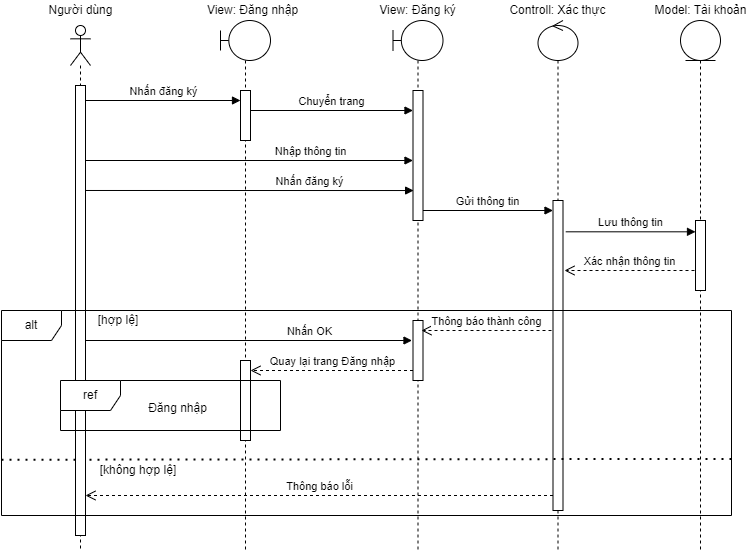
\includegraphics[width=11cm,height=13.5cm]{Images/sequence/sequence_register.png}
  \caption[Sơ đồ tuần tự chức năng đăng ký tài khoản]{\bfseries \fontsize{12pt}{0pt}
  \selectfont Sơ đồ tuần tự chức năng đăng ký tài khoản}
  \label{sequence_register} %đặt tên cho ảnh
\end{figure}
Sơ đồ tuần tự trên mô tả chi tiết quá trình người dùng đăng ký tài khoản trên hệ thống. Người dùng sẽ gửi yêu cầu đăng ký, yêu cầu sẽ được xử lý
bởi lớp Register, nếu có lỗi phát sinh sẽ hiển thị lên màn hình và yêu cầu người dùng nhập lại. Nếu việc đăng ký thành công, lớp Register sẽ gửi thông báo 
chuyển sang phê duyệt tài khoản và thông báo kết quả.  

\subsubsection{Sơ đồ tuần tự chức năng đăng nhập/đăng xuất}
\begin{figure}[H]
  \centering
  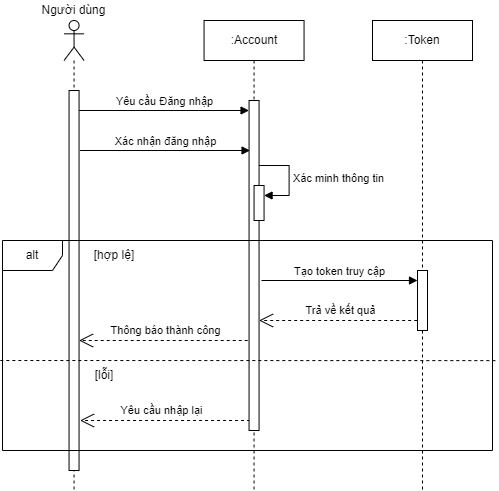
\includegraphics[width=13cm,height=12cm]{Images/sequence/sequence_login.png}
  \caption[Sơ đồ tuần tự chức năng đăng nhập]{\bfseries \fontsize{12pt}{0pt}
  \selectfont Sơ đồ tuần tự chức năng đăng nhập}
  \label{sequence_login} %đặt tên cho ảnh
\end{figure}
Sơ đồ tuần tự trên mô tả chi tiết quá trình người dùng đăng nhập trên hệ thống. Người dùng sẽ gửi yêu cầu đăng nhập, yêu cầu sẽ được xử lý
bởi lớp Account, nếu có lỗi phát sinh sẽ hiển thị lên màn hình và yêu cầu người dùng nhập lại. Nếu việc đăng ký thành công, lớp Account sẽ gửi thông báo 
tạo token truy cập mới và thông báo thành công. 
\begin{figure}[H]
  \centering
  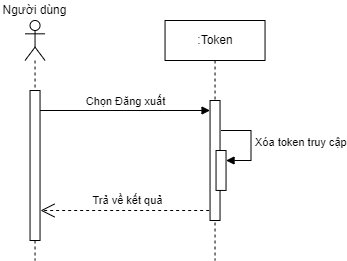
\includegraphics[width=10cm,height=7cm]{Images/sequence/sequence_logout.png}
  \caption[Sơ đồ tuần tự chức năng đăng xuất]{\bfseries \fontsize{12pt}{0pt}
  \selectfont Sơ đồ tuần tự chức năng đăng xuất}
  \label{sequence_logout} %đặt tên cho ảnh
\end{figure}
Sơ đồ tuần tự trên mô tả chi tiết quá trình người dùng đăng xuất khỏi hệ thống. Người dùng sẽ gửi yêu cầu đăng xuất, yêu cầu sẽ được xử lý
bởi lớp Token. Lớp Token sẽ xóa thông tin token truy cập và trả về kết quả đăng xuất.

\subsubsection{Sơ đồ tuần tự chức năng quên mật khẩu}
\begin{figure}[H]
  \centering
  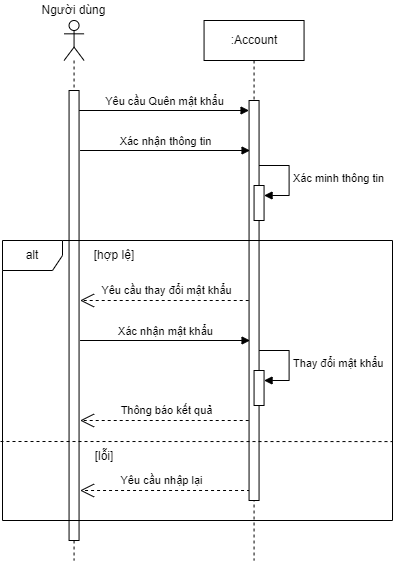
\includegraphics[width=10.5cm,height=14cm]{Images/sequence/sequence_forgot_password.png}
  \caption[Sơ đồ tuần tự chức năng quên mật khẩu]{\bfseries \fontsize{12pt}{0pt}
  \selectfont Sơ đồ tuần tự chức năng quên mật khẩu}
  \label{sequence_forgot_pass} %đặt tên cho ảnh
\end{figure}
Sơ đồ tuần tự trên mô tả chi tiết quá trình người dùng thay đổi mật khẩu trên hệ thống. Người dùng sẽ gửi nhập email đã đăng ký tài khoản, gửi yêu cầu
lấy lại mật khẩu. Yêu cầu sẽ được xử lý bởi lớp Account, nếu có lỗi phát sinh sẽ hiển thị lên màn hình và yêu cầu người dùng nhập lại. Lớp Account sẽ gửi một mã xác thực
đến email, người dùng sẽ nhập mã xác thực và thay đổi mật khẩu mới. Nếu việc thay đổi thành công, lớp Account sẽ gửi thông báo thành công và chuyển sang đăng nhập.

\subsubsection{Sơ đồ tuần tự chức năng quản lý tài khoản cá nhân}
\begin{figure}[H]
  \centering
  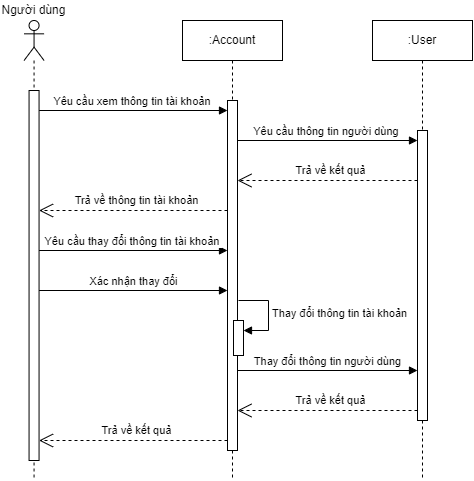
\includegraphics[width=13cm,height=13cm]{Images/sequence/sequence_manage_info.png}
  \caption[Sơ đồ tuần tự chức năng quản lý tài khoản cá nhân]{\bfseries \fontsize{12pt}{0pt}
  \selectfont Sơ đồ tuần tự chức năng quản lý tài khoản cá nhân}
  \label{sequence_account} %đặt tên cho ảnh
\end{figure}
Sơ đồ tuần tự trên mô tả chi tiết quá trình người dùng xem và thay đổi thông tin tài khoản trên hệ thống. Người dùng thay đổi thông tin và gửi yêu cầu, 
yêu cầu sẽ được xử lý bởi lớp Account và User, nếu có lỗi phát sinh sẽ hiển thị lên màn hình và yêu cầu người dùng nhập lại. Nếu việc thay đổi thành công, lớp Account sẽ gửi thông báo 
thành công.  

\subsubsection{Sơ đồ tuần tự chức năng quản lý dữ liệu đo}
\begin{figure}[H]
  \centering
  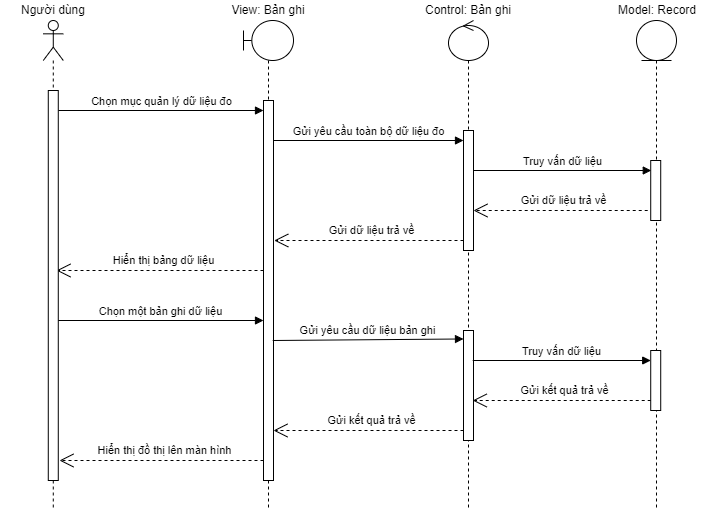
\includegraphics[width=10cm,height=7cm]{Images/sequence/sequence_manage_record.png}
  \caption[Sơ đồ tuần tự chức năng xem danh sách lịch sử đo]{\bfseries \fontsize{12pt}{0pt}
  \selectfont Sơ đồ tuần tự chức năng xem danh sách lịch sử đo}
  \label{sequence_manage_record} %đặt tên cho ảnh
\end{figure}
Sơ đồ tuần tự trên mô tả chi tiết quá trình người dùng xem danh sách lịch sử đo trên hệ thống. Người dùng chọn mở giao diện quản lý dữ liệu đo, 
yêu cầu sẽ được xử lý bởi lớp Record, hiện danh sách các bản ghi phiên đo cho người dùng.

\begin{figure}[H]
  \centering
  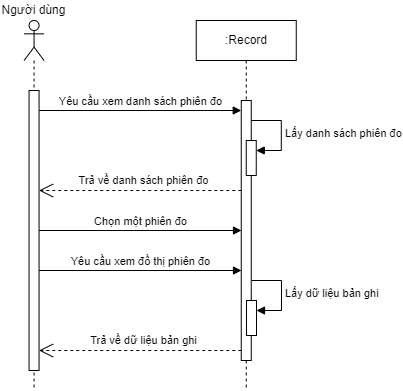
\includegraphics[width=11cm,height=10.5cm]{Images/sequence/sequence_manage_chart_record.png}
  \caption[Sơ đồ tuần tự chức năng xem đồ thị phiên đo]{\bfseries \fontsize{12pt}{0pt}
  \selectfont Sơ đồ tuần tự chức năng xem đồ thị phiên đo}
  \label{sequence_manage_chart_record} %đặt tên cho ảnh
\end{figure}
Sơ đồ tuần tự trên mô tả chi tiết quá trình người dùng xem đồ thị phiên đo trên hệ thống. Người dùng chọn một phiên đo sau đó yêu cầu xem đồ thị, 
yêu cầu sẽ được xử lý bởi lớp Record, hiện đồ thị phiên đo cho người dùng.

\begin{figure}[H]
  \centering
  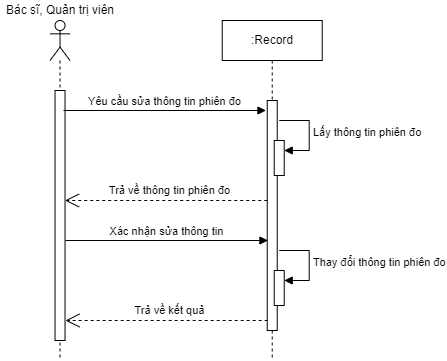
\includegraphics[width=11cm,height=9.5cm]{Images/sequence/sequence_manage_edit_record.png}
  \caption[Sơ đồ tuần tự chức năng sửa thông tin phiên đo]{\bfseries \fontsize{12pt}{0pt}
  \selectfont Sơ đồ tuần tự chức năng sửa thông tin phiên đo}
  \label{sequence_edit_record} %đặt tên cho ảnh
\end{figure}
Nếu bác sĩ, quản trị viên muốn sửa thông tin phiên đo, bác sĩ và quản trị viên gửi yêu cầu thay đổi, yêu cầu sẽ được xử lý bởi lớp Record, 
nếu có lỗi phát sinh sẽ hiển thị lên màn hình, nếu thay đổi thành công lớp Record sẽ gửi thông báo thành công. 

\begin{figure}[H]
  \centering
  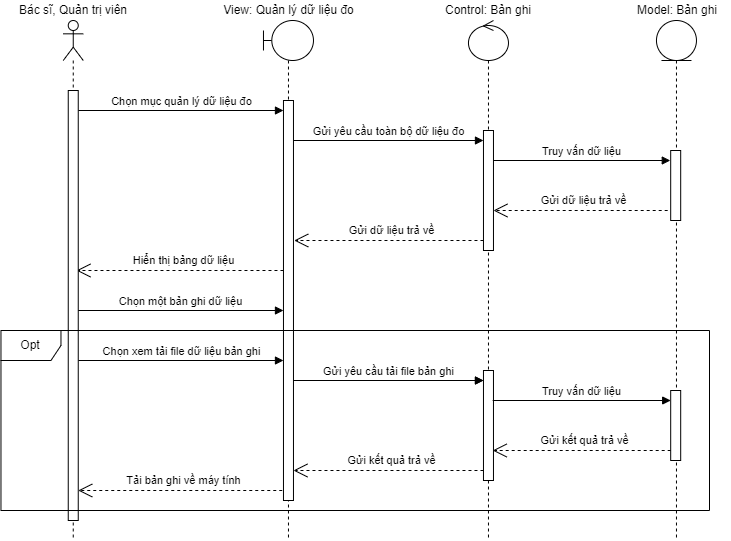
\includegraphics[width=11cm,height=9.5cm]{Images/sequence/sequence_download_records.png}
  \caption[Sơ đồ tuần tự chức năng tải bản ghi dữ liệu đo]{\bfseries \fontsize{12pt}{0pt}
  \selectfont Sơ đồ tuần tự chức năng tải bản ghi dữ liệu đo}
  \label{sequence_download_record} %đặt tên cho ảnh
\end{figure}
Nếu bác sĩ, quản trị viên muốn tải bản ghi dữ liệu đo, bác sĩ và quản trị viên gửi yêu cầu tải, yêu cầu sẽ được xử lý bởi lớp Record, 
nếu có lỗi phát sinh sẽ hiển thị lên màn hình, nếu thay đổi thành công lớp Record sẽ gửi file về máy tính. 
\subsubsection{Sơ đồ tuần tự chức năng quản lý dịch vụ nhắn tin}
\begin{figure}[H]
  \centering
  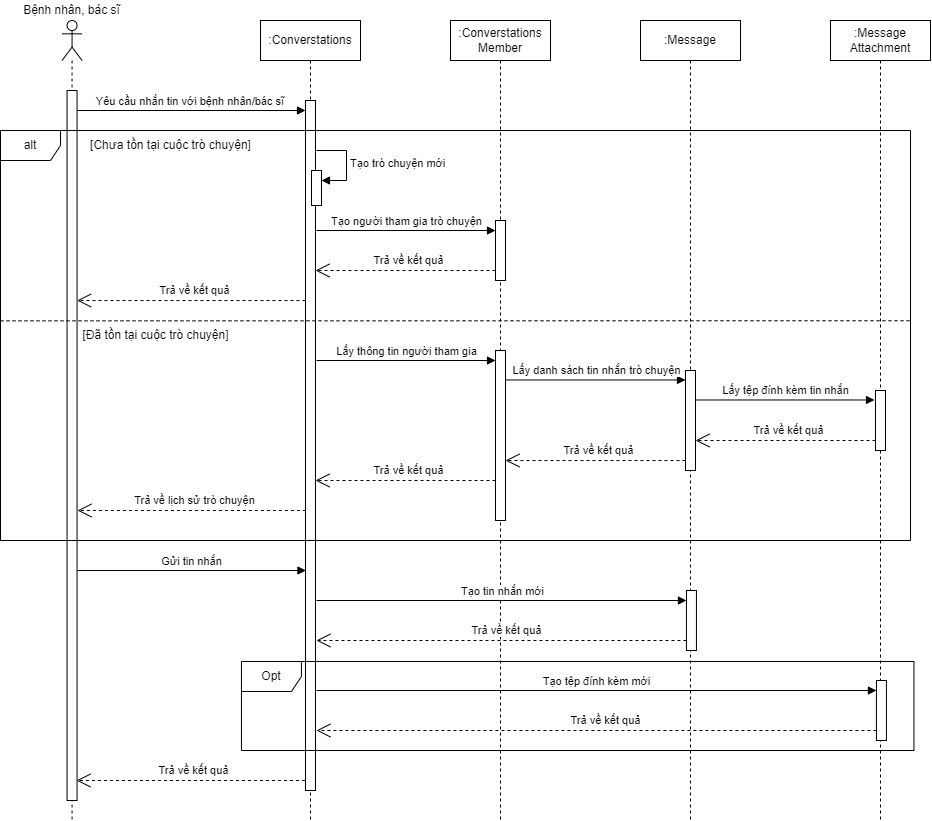
\includegraphics[width=15cm,height=13.5cm]{Images/sequence/sequence_chat.png}
  \caption[Sơ đồ tuần tự chức năng quản lý dịch vụ nhắn tin]{\bfseries \fontsize{12pt}{0pt}
  \selectfont Sơ đồ tuần tự chức năng quản lý dịch vụ nhắn tin}
  \label{sequence_chat} %đặt tên cho ảnh
\end{figure}
Sơ đồ tuần tự trên mô tả chi tiết quá trình người dùng xem và gửi tin nhắn giữa bệnh nhân và bác sĩ trên hệ thống. Người dùng gửi yêu cầu nhắn tin, 
chọn người mà mình muốn xem/gửi tin nhắn. Khi đó yêu cầu sẽ được xử lý bởi lớp Conversation, nếu bạn đã có hội thoại sẽ trả về lịch sử đoạn hội thoại, ngược lại bạn sẽ tạo cuộc hội thoại mới. 
Nếu người dùng gửi tin nhắn, yêu cầu sẽ được xử lý bởi lớp Conversation gửi tin nhắn đến đối phương và lưu vào cơ sở dữ liệu.

\subsubsection{Sơ đồ tuần tự chức năng hỏi, nhận tư vấn từ trợ lý ảo}
\begin{figure}[H]
  \centering
  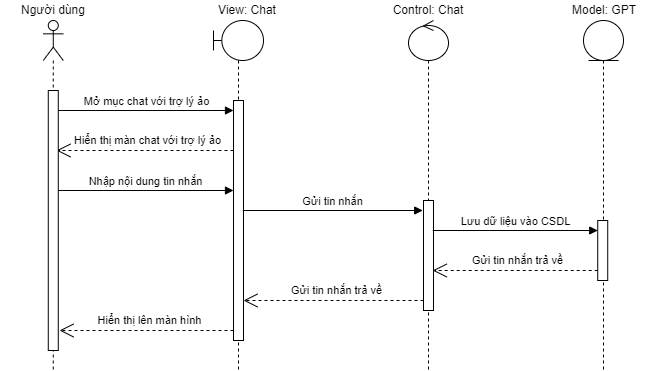
\includegraphics[width=14.5cm,height=10cm]{Images/sequence/sequence_chat_ai.png}
  \caption[Sơ đồ tuần tự chức năng hỏi, nhận tư vấn từ trợ lý ảo]{\bfseries \fontsize{12pt}{0pt}
  \selectfont Sơ đồ tuần tự chức năng hỏi, nhận tư vấn từ trợ lý ảo}
  \label{sequence_chat_ai} %đặt tên cho ảnh
\end{figure}
Sơ đồ tuần tự trên mô tả chi tiết quá trình người dùng xem và gửi tin nhắn với trợ lý ảo trên hệ thống. Người dùng chọn mở giao diện nhắn tin với trợ lý ảo, 
khi người dùng gửi tin nhắn đến trợ lý ảo, yêu cầu sẽ được xử lý bởi lớp Conversation gửi đến trợ lý ảo và phản hồi lại câu trả lời từ trợ lý ảo.

\subsubsection{Sơ đồ tuần tự chức năng quản lý thiết bị}
\begin{figure}[H]
  \centering
  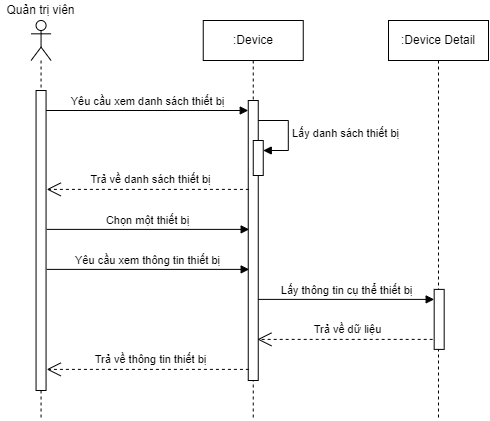
\includegraphics[width=13cm,height=11cm]{Images/sequence/sequence_manage_device.png}
  \caption[Sơ đồ tuần tự chức năng xem danh sách thiết bị]{\bfseries \fontsize{12pt}{0pt}
  \selectfont Sơ đồ tuần tự chức năng xem danh sách thiết bị}
  \label{sequence_manage_device} %đặt tên cho ảnh
\end{figure}
Sơ đồ tuần tự trên mô tả chi tiết quá trình quản trị viên xem danh sách thiết bị trên hệ thống. Quản trị viên chọn mở giao diện quản lý thiết bị, 
API sẽ được xử lý bởi lớp Device, hiện danh sách thiết bị, quản trị viên có thể chọn một thiết bị và xem thông tin của họ. 
\begin{figure}[H]
  \centering
  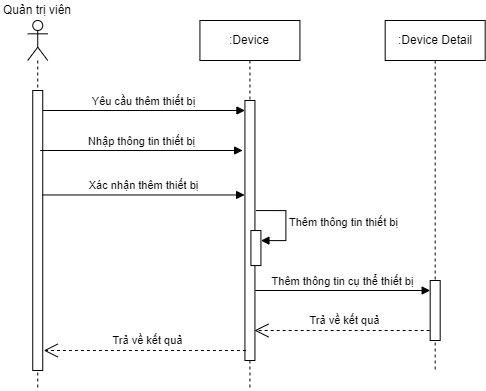
\includegraphics[width=13cm,height=10cm]{Images/sequence/sequence_manage_add_device.png}
  \caption[Sơ đồ tuần tự chức năng thêm thiết bị]{\bfseries \fontsize{12pt}{0pt}
  \selectfont Sơ đồ tuần tự chức năng thêm thiết bị}
  \label{sequence_manage_add_device} %đặt tên cho ảnh
\end{figure}
Nếu quản trị viên muốn tạo một thiết bị mới, quản trị viên nhập các thông tin và gửi yêu cầu tạo, yêu cầu sẽ được xử lý bởi lớp Device, nếu có lỗi phát sinh sẽ hiển thị lên màn hình, 
nếu tạo thành công lớp Device sẽ gửi kết quả trả về. 
\begin{figure}[H]
  \centering
  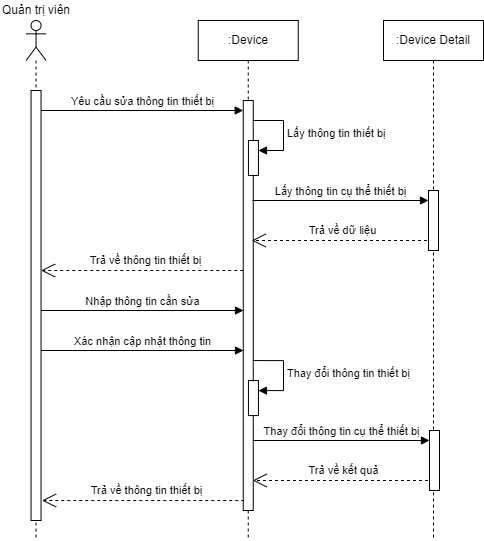
\includegraphics[width=13cm,height=12.5cm]{Images/sequence/sequence_manage_edit_device.png}
  \caption[Sơ đồ tuần tự chức năng sửa thông tin thiết bị]{\bfseries \fontsize{12pt}{0pt}
  \selectfont Sơ đồ tuần tự chức năng sửa thông tin thiết bị}
  \label{sequence_manage_edit_device} %đặt tên cho ảnh
\end{figure}
Nếu quản trị viên muốn chỉnh sửa thông tin thiết bị, quản trị viên nhập các thông tin cần sửa và gửi yêu cầu thay đổi, yêu cầu sẽ được xử lý
bởi lớp Device, nếu có lỗi phát sinh sẽ hiển thị lên màn hình, nếu thay đổi thành công Control sẽ gửi thông báo thành công. 
\begin{figure}[H]
  \centering
  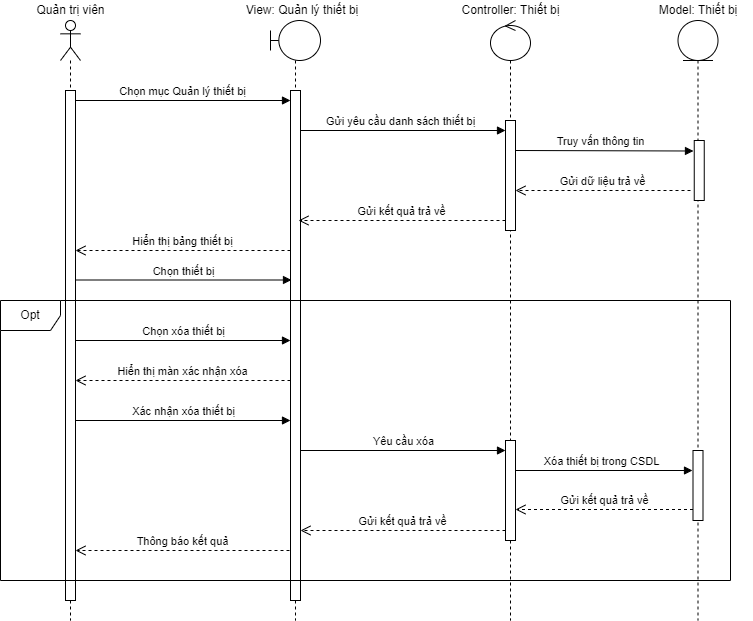
\includegraphics[width=13cm,height=10cm]{Images/sequence/sequence_manage_delete_device.png}
  \caption[Sơ đồ tuần tự chức năng xóa thiết bị]{\bfseries \fontsize{12pt}{0pt}
  \selectfont Sơ đồ tuần tự chức năng xóa thiết bị}
  \label{sequence_manage_delete_device} %đặt tên cho ảnh
\end{figure}
Nếu quản trị viên yêu cầu xóa thiết bị, lớp Device sẽ xử lý xóa thiết bị ở cơ sở dữ liệu và trả về thông báo cho quản trị viên.


\subsubsection{Sơ đồ tuần tự chức năng quản lý phân công bác sĩ - bệnh nhân}
\begin{figure}[H]
  \centering
  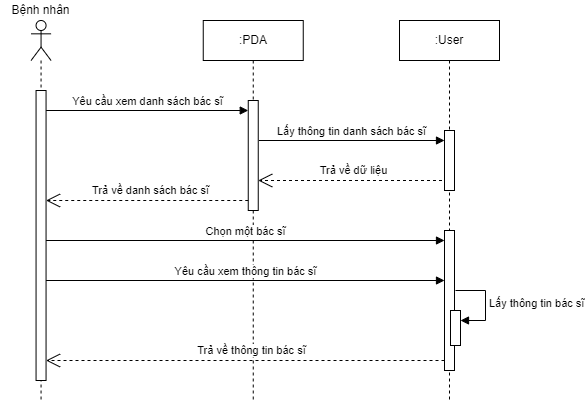
\includegraphics[width=13cm,height=9.5cm]{Images/sequence/sequence_manage_doctor.png}
  \caption[Sơ đồ tuần tự chức năng xem danh sách bác sĩ]{\bfseries \fontsize{12pt}{0pt}
  \selectfont Sơ đồ tuần tự chức năng xem danh sách bác sĩ}
  \label{sequence_manage_doctor} %đặt tên cho ảnh
\end{figure}
Sơ đồ tuần tự trên mô tả chi tiết quá trình bệnh nhân xem danh sách bác sĩ phụ trách mình trên hệ thống. Bệnh nhân chọn mở giao diện xem danh sách bác sĩ, 
yêu cầu sẽ được xử lý bởi lớp PDA, hiện danh sách bác sĩ, bệnh nhân có thể chọn một bác sĩ và xem thông tin của họ. 
\begin{figure}[H]
  \centering
  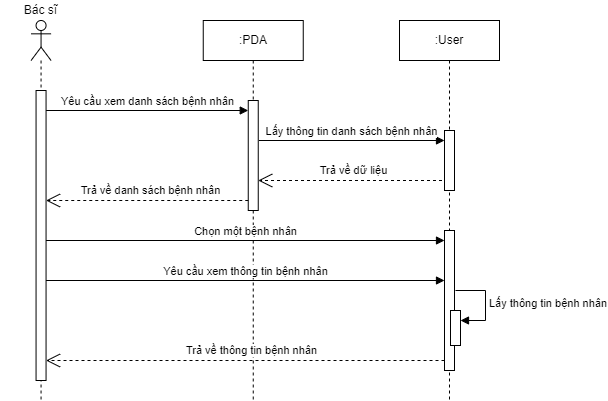
\includegraphics[width=13cm,height=9.5cm]{Images/sequence/sequence_manage_patient.png}
  \caption[Sơ đồ tuần tự chức năng xem danh sách bệnh nhân]{\bfseries \fontsize{12pt}{0pt}
  \selectfont Sơ đồ tuần tự chức năng xem danh sách bệnh nhân}
  \label{sequence_manage_patient} %đặt tên cho ảnh
\end{figure}
Sơ đồ tuần tự trên mô tả chi tiết quá trình bác sĩ xem danh sách bệnh nhân trên hệ thống. Bác sĩ chọn mở giao diện xem danh sách bệnh nhân, 
yêu cầu sẽ được xử lý bởi lớp PDA, hiện danh sách bệnh nhân, bác sĩ có thể chọn một bệnh nhân và xem thông tin của họ. 

\begin{figure}[H]
  \centering
  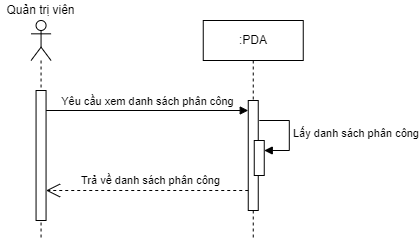
\includegraphics[width=11cm,height=8cm]{Images/sequence/sequence_manage_pda.png}
  \caption[Sơ đồ tuần tự chức năng xem danh sách phân công bác sĩ - bệnh nhân]{\bfseries \fontsize{12pt}{0pt}
  \selectfont Sơ đồ tuần tự chức năng xem danh sách phân công bác sĩ - bệnh nhân}
  \label{sequence_manage_pda} %đặt tên cho ảnh
\end{figure}
Sơ đồ tuần tự trên mô tả chi tiết quá trình quản trị viên xem danh sách phân công bác sĩ - bệnh nhân trên hệ thống. Quản trị viên chọn mở giao diện
quản lý phân công bác sĩ - bệnh nhân, yêu cầu sẽ được xử lý bởi lớp PDA, hiện danh sách phân công bác sĩ - bệnh nhân. 

\begin{figure}[H]
  \centering
  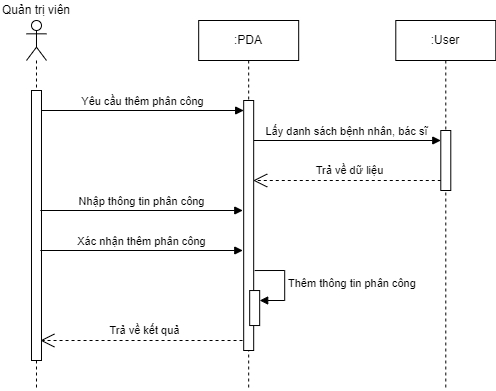
\includegraphics[width=13cm,height=10cm]{Images/sequence/sequence_manage_add_pda.png}
  \caption[Sơ đồ tuần tự chức năng thêm phân công bác sĩ - bệnh nhân]{\bfseries \fontsize{12pt}{0pt}
  \selectfont Sơ đồ tuần tự chức năng thêm phân công bác sĩ - bệnh nhân}
  \label{sequence_manage_add_pda} %đặt tên cho ảnh
\end{figure}
Sơ đồ tuần tự trên mô tả chi tiết quá trình quản trị viên tạo với danh sách phân công bác sĩ - bệnh nhân trên hệ thống. Quản trị viên chọn mở giao diện
quản lý phân công bác sĩ - bệnh nhân, yêu cầu sẽ được xử lý bởi lớp PDA, hiện danh sách phân công bác sĩ - bệnh nhân. 

\begin{figure}[H]
  \centering
  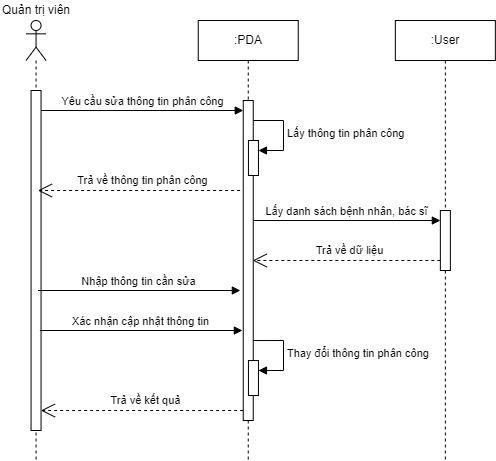
\includegraphics[width=13cm,height=12cm]{Images/sequence/sequence_manage_edit_pda.png}
  \caption[Sơ đồ tuần tự chức năng sửa thông tin phân công bác sĩ - bệnh nhân]{\bfseries \fontsize{12pt}{0pt}
  \selectfont Sơ đồ tuần tự chức năng sửa thông tin phân công bác sĩ - bệnh nhân}
  \label{sequence_manage_edit_pda} %đặt tên cho ảnh
\end{figure}
Nếu quản trị viên muốn chỉnh sửa thông tin phân công bác sĩ - bệnh nhân, quản trị viên nhập các thông tin cần sửa và gửi yêu cầu thay đổi, 
yêu cầu sẽ được xử lý bởi lớp PDA, nếu có lỗi phát sinh sẽ hiển thị lên màn hình, nếu thay đổi thành công Control sẽ gửi thông báo thành công. 
\begin{figure}[H]
  \centering
  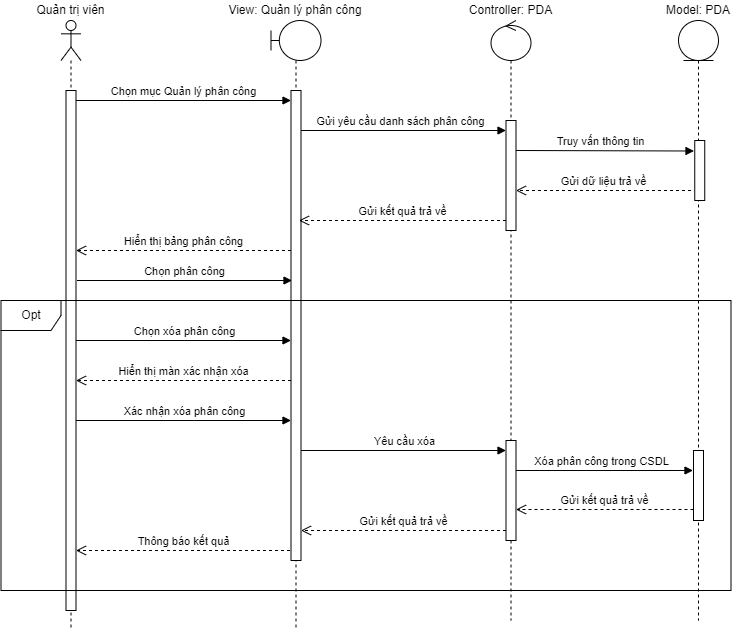
\includegraphics[width=11cm,height=8.5cm]{Images/sequence/sequence_manage_delete_pda.png}
  \caption[Sơ đồ tuần tự chức năng xóa phân công bác sĩ - bệnh nhân]{\bfseries \fontsize{12pt}{0pt}
  \selectfont Sơ đồ tuần tự chức năng xóa phân công bác sĩ - bệnh nhân}
  \label{sequence_manage_delete_pda} %đặt tên cho ảnh
\end{figure}
Nếu quản trị viên yêu cầu xóa phân công bác sĩ - bệnh nhân, Control sẽ xử lý xóa phân công ở cơ sở dữ liệu và trả về thông báo cho quản trị viên.

\subsubsection{Sơ đồ tuần tự chức năng quản lý tài khoản người dùng}
\begin{figure}[H]
  \centering
  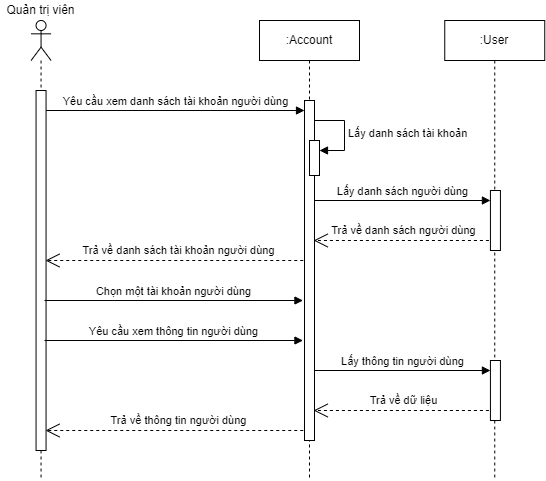
\includegraphics[width=13cm,height=11cm]{Images/sequence/sequence_manage_user.png}
  \caption[Sơ đồ tuần tự chức năng xem danh sách tài khoản người dùng]{\bfseries \fontsize{12pt}{0pt}
  \selectfont Sơ đồ tuần tự chức năng xem danh sách tài khoản người dùng}
  \label{sequence_manage_user} %đặt tên cho ảnh
\end{figure}
Sơ đồ tuần tự trên mô tả chi tiết quá trình quản trị viên xem danh sách tài khoản người dùng trên hệ thống. Quản trị viên yêu cầu xem
quản lý tài khoản người dùng, yêu cầu sẽ được xử lý bởi lớp User, trả về danh sách tài khoản người dùng, quản trị viên có thể chọn một người dùng và xem thông tin của họ. 
\begin{figure}[H]
  \centering
  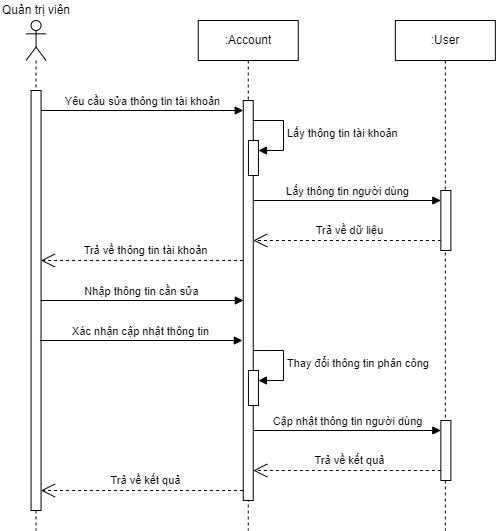
\includegraphics[width=13cm,height=13cm]{Images/sequence/sequence_manage_edit_user.png}
  \caption[Sơ đồ tuần tự chức năng sửa thông tin người dùng]{\bfseries \fontsize{12pt}{0pt}
  \selectfont Sơ đồ tuần tự chức năng sửa thông tin người dùng}
  \label{sequence_manage_edit_user} %đặt tên cho ảnh
\end{figure}
Nếu quản trị viên muốn chỉnh sửa thông tin người dùng, quản trị viên nhập các thông tin cần sửa và gửi yêu cầu thay đổi, yêu cầu sẽ được xử lý bởi lớp User, nếu có lỗi phát sinh sẽ hiển thị lên màn hình,
nếu thay đổi thành công lớp User sẽ gửi thông báo thành công. 
\begin{figure}[H]
  \centering
  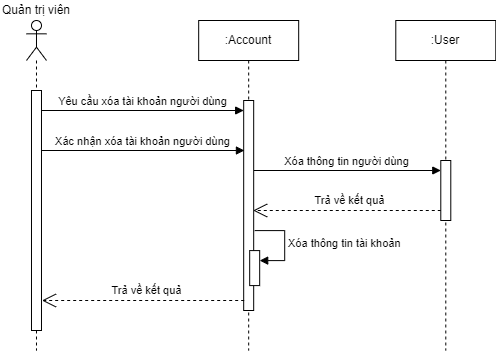
\includegraphics[width=11cm,height=8.5cm]{Images/sequence/sequence_manage_delete_user.png}
  \caption[Sơ đồ tuần tự chức năng xóa người dùng]{\bfseries \fontsize{12pt}{0pt}
  \selectfont Sơ đồ tuần tự chức năng xóa người dùng}
  \label{sequence_manage_delete_user} %đặt tên cho ảnh
\end{figure}
Nếu quản trị viên yêu cầu xóa tài khoản người dùng, lớp User sẽ xử lý xóa tài khoản ở cơ sở dữ liệu và trả về thông báo cho quản trị viên.
\begin{figure}[H]
  \centering
  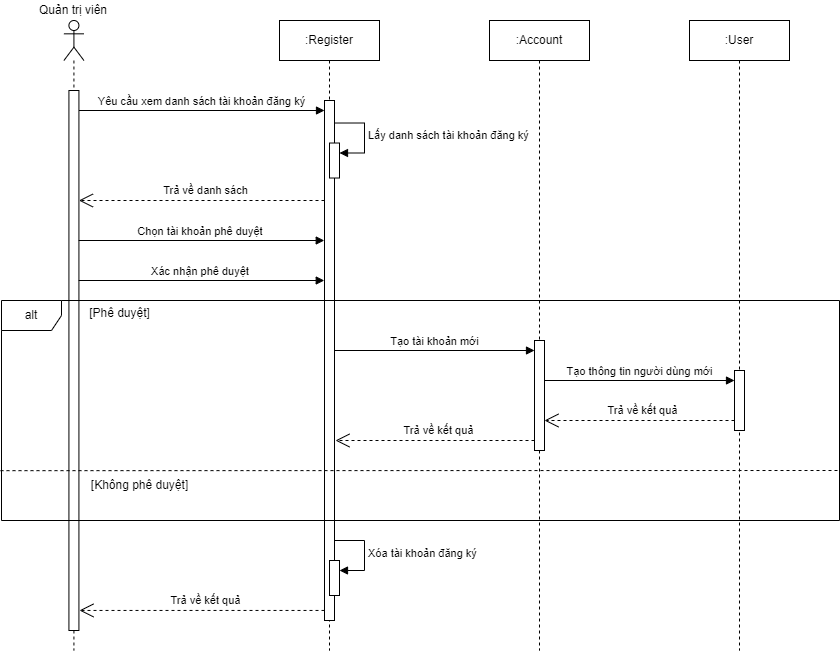
\includegraphics[width=14.5cm,height=13cm]{Images/sequence/sequence_manage_register.png}
  \caption[Sơ đồ tuần tự chức năng phê duyệt tài khoản người dùng]{\bfseries \fontsize{12pt}{0pt}
  \selectfont Sơ đồ tuần tự chức năng phê duyệt tài khoản người dùng}
  \label{sequence_manage_register} %đặt tên cho ảnh
\end{figure}
Nếu quản trị viên muốn phê duyệt tài khoản người dùng, quản trị sẽ chọn phê duyệt hoặc không phê duyệt, yêu cầu sẽ được xử lý bởi lớp Register, nếu có lỗi phát sinh sẽ hiển thị lên màn hình,
nếu phê duyệt thành công lớp Register sẽ gửi thông báo thành công. 

\subsection{Phân tích dữ liệu}

Tại phần này, chúng em sẽ tiến hành xác định và mô tả các thực thể cũng như
 thuộc tính quan trọng trong hệ thống. Việc này giúp chúng ta có cái
  nhìn tổng quan về các yếu tố chính cần được quản lý và lưu trữ
   trong cơ sở dữ liệu. Bằng cách làm điều này, chúng ta có thể
    xây dựng một mô hình dữ liệu cơ bản để hỗ trợ việc thiết kế và
     triển khai hệ thống một cách hiệu quả.

     Trước hết, chúng em sẽ xác định và mô tả các thực thể chính trong hệ
      thống. Thực thể là các đối tượng hoặc khái niệm quan
       trọng mà chúng ta cần theo dõi và quản lý. Sau đó, chúng ta sẽ xác
        định các thuộc tính liên quan đến mỗi thực thể, các thông tin cần
         được lưu trữ và quản lý.

\begin{table}[H]
  \caption{\bfseries \fontsize{12pt}{0pt}\selectfont Bảng thực thể và thuộc tính}
  \centering
  \begin{tabularx}{0.9\textwidth}{|c|X|}
    \hline
    \textbf{Thực thể} & \textbf{Thuộc tính} \\
    \hline
    Người dùng & 
    ID người dùng, ID tài khoản, Tên người dùng, Ngày sinh, Giới tính, Số điện thoại, Quyền, Trạng thái, Đường dẫn lưu trữ ảnh, Thông tin người dùng \\
    \hline
    Tài khoản &
    ID tài khoản, Email, Mật khẩu  \\
    \hline
    Token đăng nhập &
    ID token, ID tài khoản, Token truy cập, Token làm mới \\
    \hline
    Thiết bị & 
    ID thiết bị, ID người dùng thiết bị, ID bác sĩ theo dõi, Tên thiết bị, Loại thiết bị, Thông tin thiết bị, Trạng thái thiết bị, Ngày bắt đầu sử dụng\\
    \hline
    Thông số thiết bị &
    ID thông số, ID thiết bị, Tên thông số, Giá trị thông số, Thông tin cụ thể, Loại thông số \\
    \hline
    Bản ghi dữ liệu & 
    ID bản ghi dữ liệu, ID người dùng, ID thiết bị, Loại bản ghi, Đường dẫn lưu trữ dữ liệu, Thời gian bắt đầu đo, Thời gian kết thúc đo \\
    \hline
    Thông tin hội thoại &
    ID hội thoại, Tên hội thoại, Loại hội thoại, Đường dẫn avatar hội thoại \\
    \hline
    Thành viên tham gia hội thoại &
    ID hội thoại, ID người dùng tham gia, Trạng thái thông báo (Có thông báo, Không thông báo), Tác vụ (người tạo đoạn hội thoại, thành viên trong đoạn hội thoại), Trạng thái đã xem\\
    \hline
    Tin nhắn & 
    ID tin nhắn, ID hội thoại, ID người gửi, Các tệp đính kèm, Tin nhắn hệ thống, Ghim (tin nhắn được ghim, không được ghim), Thời gian ghim tin nhắn, Các lượt thả cảm xúc \\
    \hline
    Tệp đính kèm &
    ID tệp đính kèm, ID tin nhắn, ID hội thoại, Đường dẫn nội dung, Tên tệp, Kích thước tệp, Đường dẫn thumbnail, Loại đính kèm (hình ảnh, video, tệp tin) \\
    \hline 
    Phân công bệnh nhân - bác sĩ & 
    ID phân công, ID bệnh nhân, ID bác sĩ, Ngày bắt đầu, Ngày kết thúc \\
    \hline
    Danh mục tin tức &
    ID danh mục tin tức, Tên danh mục tin tức, Mô tả danh mục tin tức \\
    \hline
    Tin tức &
    ID tin tức, Tiêu đề, Nội dung, ID danh mục tin tức, Tác giả, Đường dẫn, Đường dẫn hình ảnh \\
    \hline
    Tài khoản phê duyệt & 
    ID tài khoản phê duyệt, Email, Mật khẩu, Tên người dùng, Ngày sinh, Giới tính, Số điện thoại, Quyền, Trạng thái, Đường dẫn lưu trữ ảnh, Thông tin người dùng \\
    \hline
  \end{tabularx}

  
\end{table}
Sau khi hoàn thành được bảng thực thể và thuộc tính, chúng em xác định được mô hình thực thể liên kết như sau:

\begin{figure}[H]
  \centering
  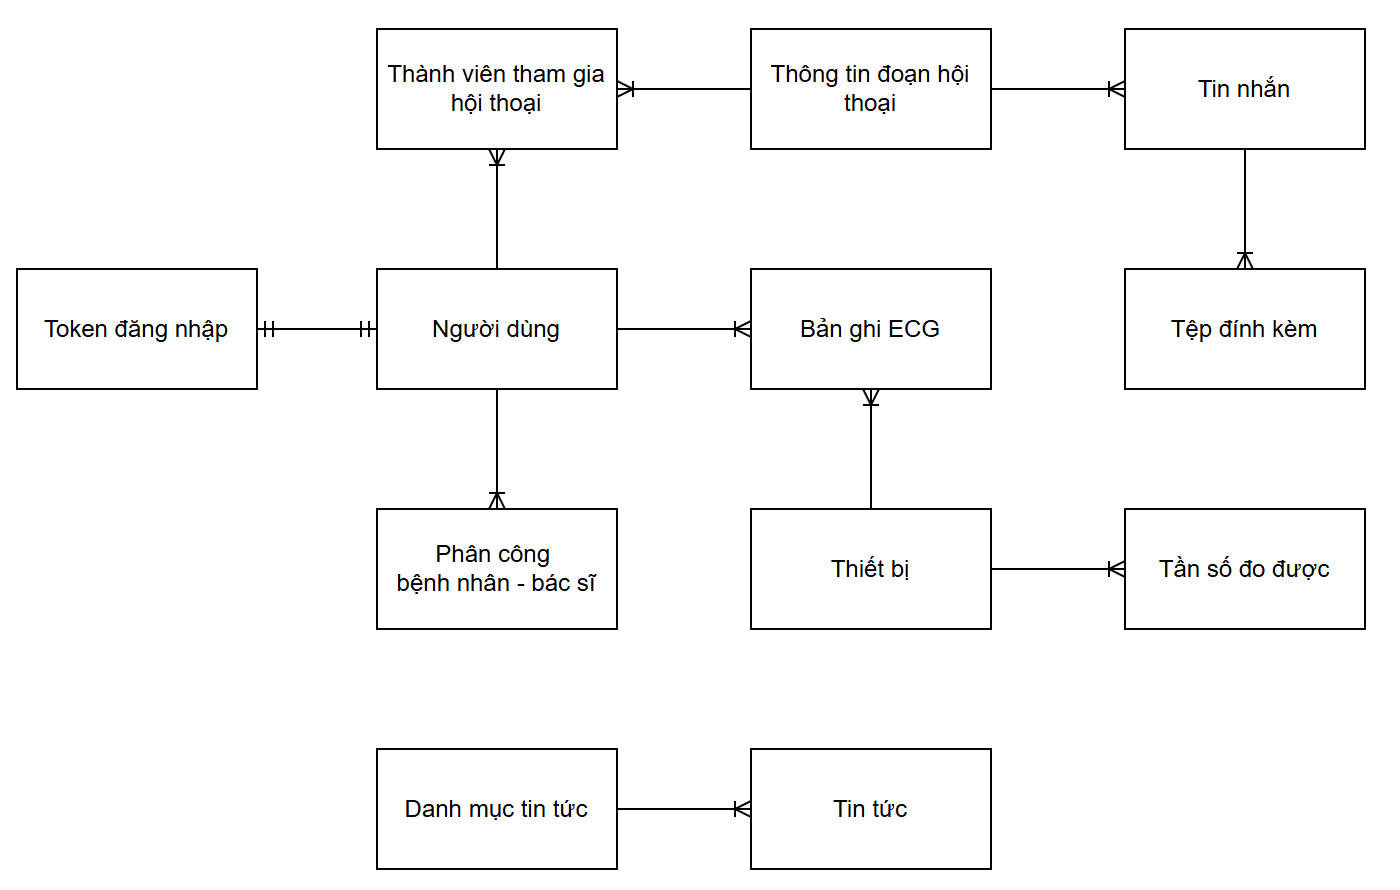
\includegraphics[width=15cm,height=9.5cm]{Images/system/fmECG_connection_entity.png}
  \caption[Mô hình thực thể liên kết]{\bfseries \fontsize{12pt}{0pt}
  \selectfont Mô hình thực thể liên kết}
  \label{ttlk} %đặt tên cho ảnh
\end{figure}

\subsection{Kết luận chương}

Trong chương này, chúng em đã thực hiện phân tích toàn diện về
 hệ thống, nhằm đáp ứng các mục tiêu và yêu cầu đã được đề xuất.

Chúng em đã xác định rõ ràng các khía cạnh quan trọng của hệ thống,
 tập trung vào việc thiết kế một hệ thống quản lý dữ liệu điện tim hiệu quả hiệu quả,
  trực quan và có khả năng theo dõi sức khỏe tim mạch một cách
   chính xác. 


\newpage
